\chapter{Влияние мутаций в белке SOD1 на время жизни пациентов с боковым амиотрофическим склерозом} \label{chapt3}

\section{Оценка стабильности водородных связей по траекториям МД} \label{sect_MD_hbonds}

\begin{figure}[ht]
  \center
  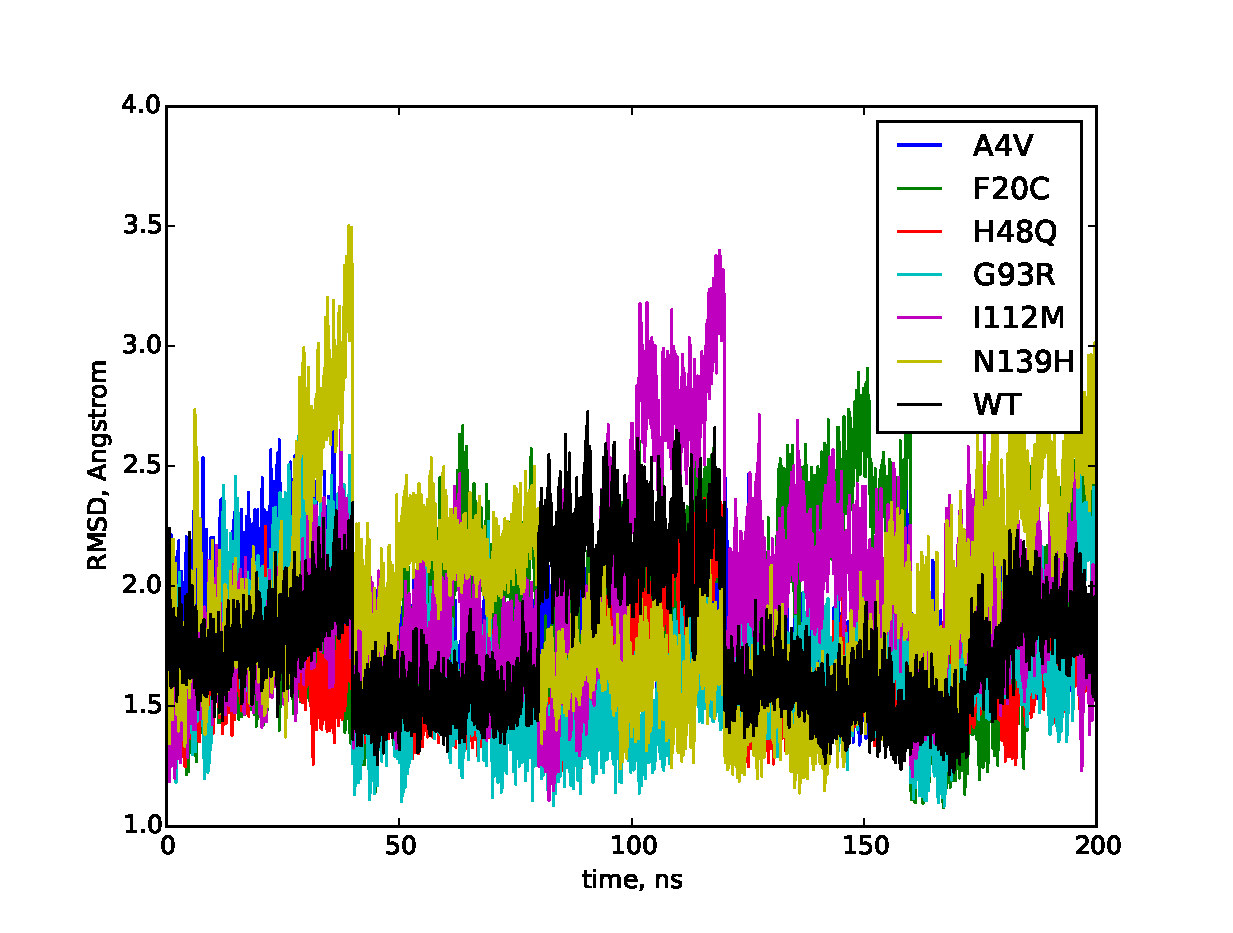
\includegraphics [width=0.75\linewidth] {md_rmsd5}
  \caption{RMSD относительно кристаллической структуры для некоторых мутантов SOD1. На общей оси абсцисс отображены результаты для всех пяти траекторий.}
  \label{img:md_hbonds}
\end{figure}

На первом шаге анализа траекторий МД для 40 димеров SOD1 (см. график RMSD на рис. \ref{img:md_hbonds}) была исследована стабильность  водородных связей между атомами белка, атомами белка и атомами молекул воды и водных мостиков (\modelpphb{}, \modelpwhb{} и \modelwbr{}, соответственно). Стабильность связей определялась как суммарное время существования соответствующей связи в течение моделирования МД, отнесённое ко всему интервалу моделирования МД. Было найдено 4386 водородных связей внутри белка, 1427 водородных связей с молекулами воды и 2268 связей, составляющих водные мостики.

% \begin{figure}[ht]
%     \center{
%         \hfill
%         \subcaptionbox[List-of-Figures entry]{Водородные связи между атомами белка.\label{img:md_bstab_a}} {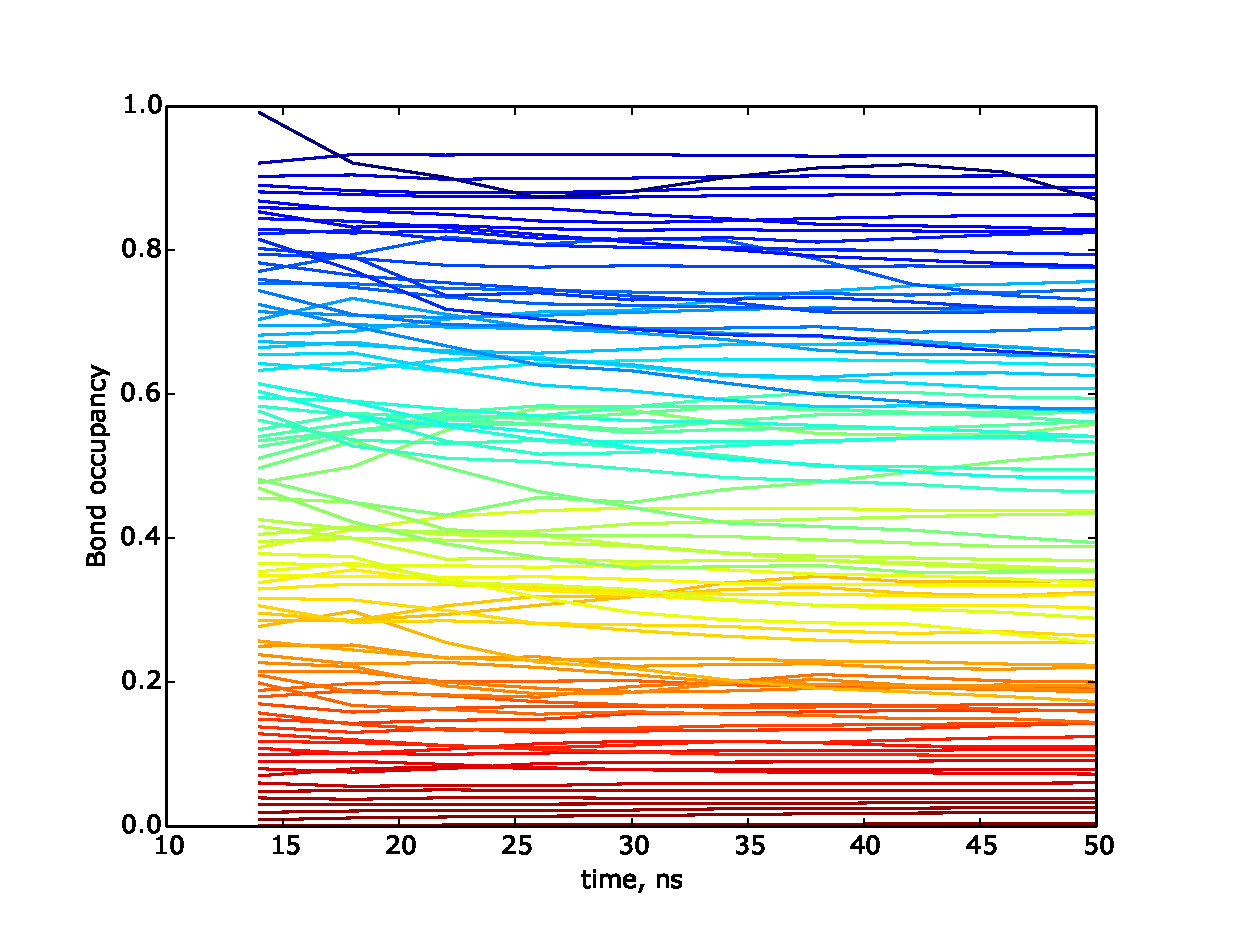
\includegraphics[width=0.75\linewidth]{md_bstab_a}}%
%         \hfill       
%         \subcaptionbox{Водородные связи между атомами белка и атомами молекул воды.\label{img:md_bstab_b}} {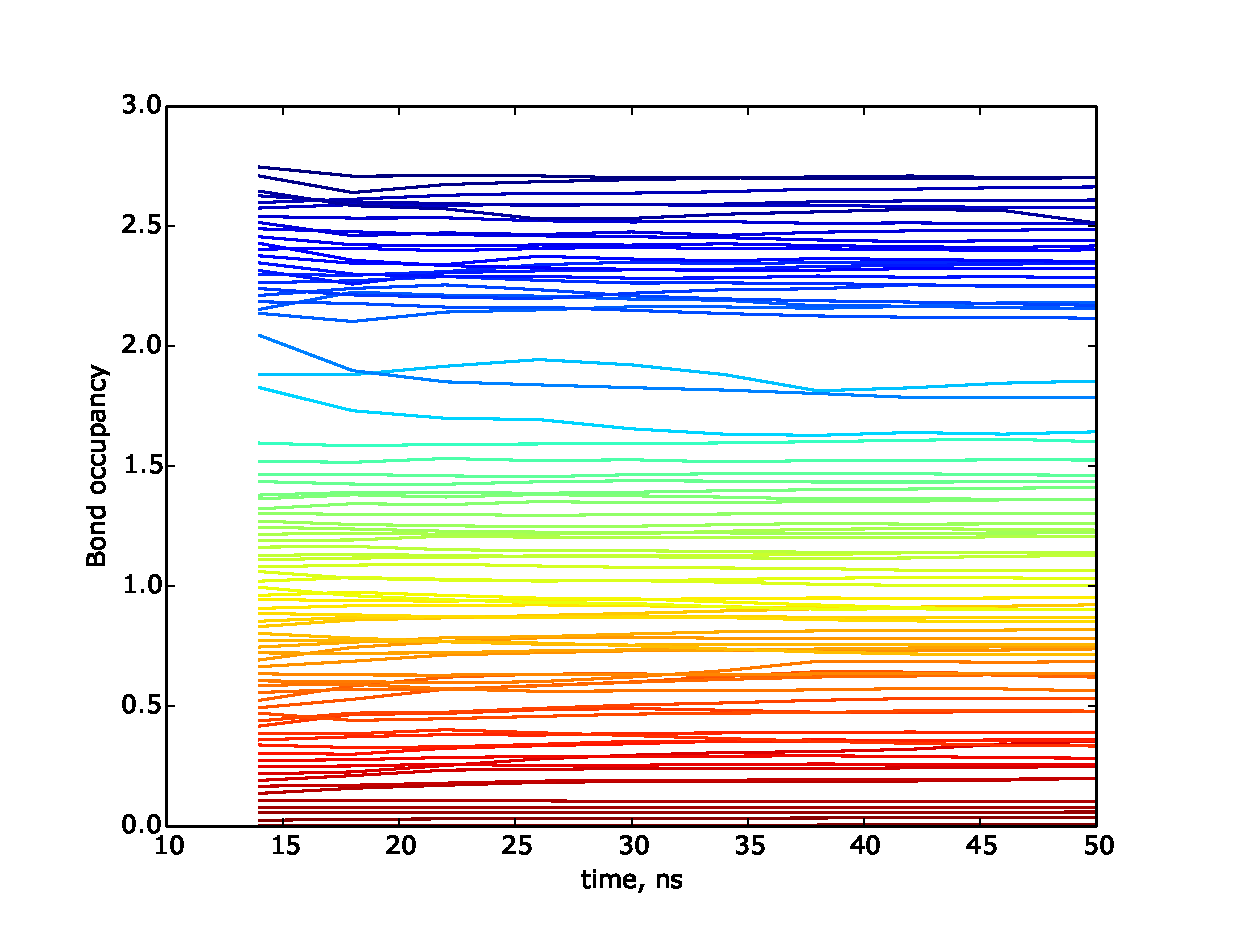
\includegraphics[width=0.75\linewidth]{md_bstab_b}}
%         \hfill
%         \subcaptionbox{Водные мостики.\label{img:md_bstab_c}} {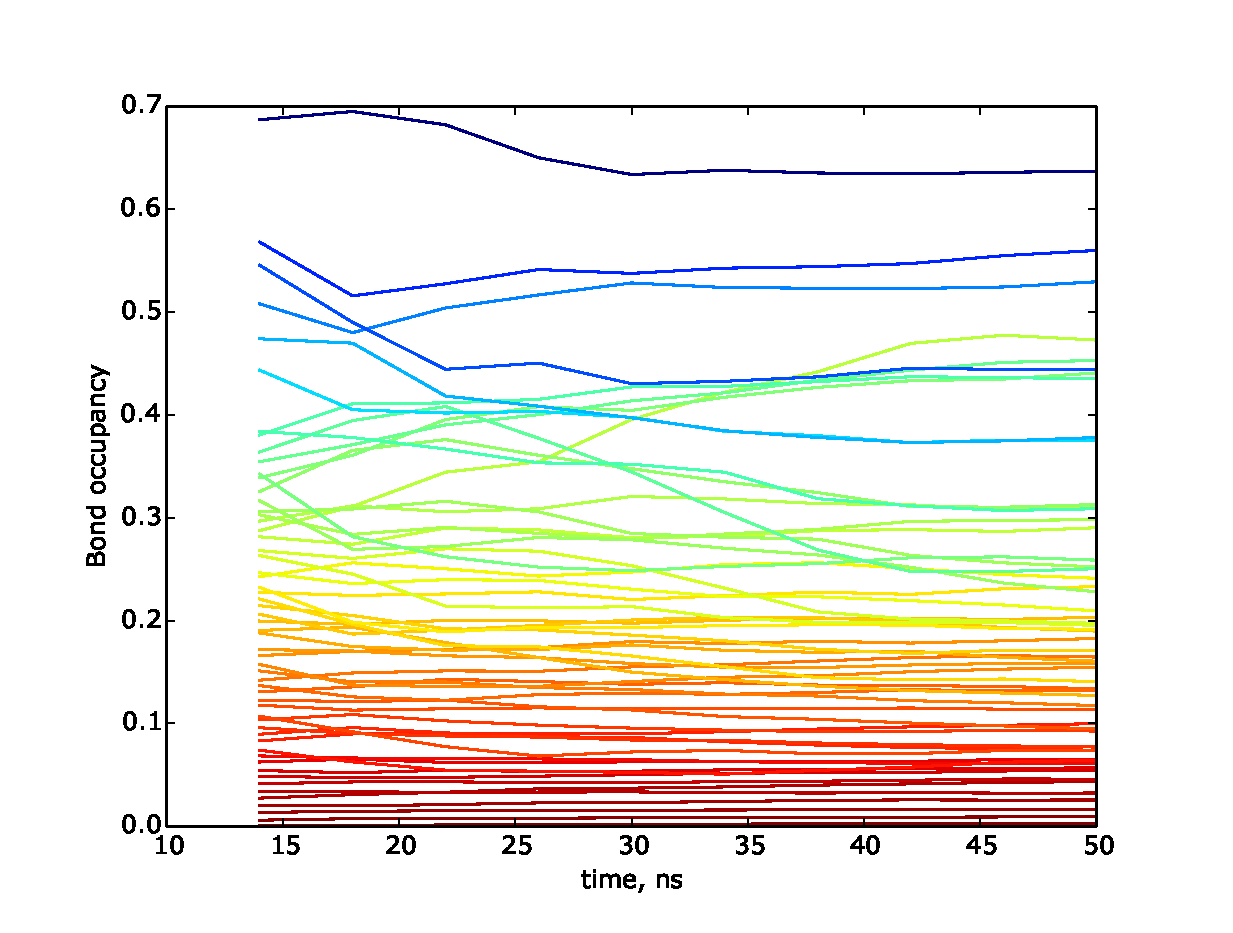
\includegraphics[width=0.75\linewidth]{md_bstab_c}}
%         \hfill
%     }
%
%     \caption{Стабильность связей различного типа между атомами моделируемой системы в зависимости от периода моделирования. Каждая линия отражает усреднённую динамику времён существования групп связей, имеющих сходную стабильность.} % Этот текст попадает в названия рисунков в списке рисунков
%     \label{img:md_bstab}
% \end{figure}

Для проверки того достаточен ли выбранный период моделирования (50 нс)  для оценки стабильности связей были построены зависимости времени существования связей от длины траектории МД. На Рис. \ref{img:md_bstab_a}, \ref{img:md_bstab_b}, \ref{img:md_bstab_c} (см. \appendixname{}~\ref{appendix:bstab}) показана динамика групп связей со схожей стабильностью. За время моделирования с 10-14 нс был определён интервал времени существования связей. Этот интервал был разбит на 30 подинтервалов, которые использовались для группировки связей. Все связи, стабильность которых попадала внутрь отдельно взятого подинтервала рассматривались как одна группа. Динамика связей для группы строилась путём усреднения стабильностей связей, входящих в данную группу. Как видно из Рис. \ref{img:md_bstab_a}, \ref{img:md_bstab_b}, \ref{img:md_bstab_c}, динамики связей при увеличении продолжительности моделирования  выходят на плато. Таким образом, выбранная длительность моделирования в 50 нс может рассматриваться достаточной для оценки стабильности связей.

\section{Построение моделей, связывающих продолжительность жизни пациентов со структурными характеристиками мутантных форм белка} \label{sect_MD_models}

Для построения модели, предсказывающей время жизни пациента, несущего определённую патологическую мутацию исследовались структурные и динамические характеристики белка. В фазовой траектории МД отслеживалось три параметра:  время существования каждой из водородных связей внутри белка, которые образовывались в процессе моделирования МД (\modelpphb{}), время существования водородных связей белка с окружающим молекулами воды (\modelpwhb{}) и время существования межатомных связей между аминокислотными остатками белка, которые образуются через взаимодействие с молекулами воды--водные мостики (\modelwbr{}).

Для каждого из параметров \modelpphb{}, \modelpwhb{} и \modelwbr{} строилась таблица, состоящая из $N$ строк и $M$ столбцов, где $N$--количество  соответствующих связей, образующихся в процессе динамики белка SOD1 (характерное $N$ в настоящем исследовании составило 1000), $M$--количество исследуемых мутаций ($M = 39$). В ячейках таблицы содержалось абсолютное значение разности между средним времемем существнвания связи с номером $n\in{\left [ 1,N \right ]}$ в процессе МД мутанта $m\in{\left [ 1,M \right ]}$ и средним временем существования связи с номером $n$ в процессе МД белка дикого типа ($T^{n,m}=\lbrace t_{n,m} \rbrace$). Усреднение проводилось по пяти независимым траекториям, расчитанным для каждой мутации.

Вторым шагом была сортировка таблицы по убыванию абсолютного значения коэффициента корреляции Пирсона между $T^{n,m}$ и продолжительностью жизни пациентов (${ST}^m$). Далее расчитывалось результирующее значение $O_{m, K}$ ($K < N$) как разница между суммой времён существования водородных связей, положительно коррелирующх с продолжительностью жизни пациентов и аналогичной суммой для отрицательно коррелирующих связей. Величина $O_{m, K}$ получалась следующим образом:

\begin{equation} \label{eq:occupancy}
O_{m, K} = \sum_{k \in \left [ 1,K \right ], R_k > 0}{T^{k, m}}-\sum_{k \in \left [ 1,K \right ], R_k < 0}{T^{k, m}}
\end{equation}

где $R_k$--коэффициент корреляции строки $\{T^{k,m}\}$ с $\{{ST}^m\}$, $K$--количество связей, удовлетворяющих условию: $R_k > R_{th}$. Для определения $R_{th}$ применялась итерационная процедура, которая максимизировала $O_{m, K}$. 

Формула \ref{eq:occupancy} отражает то, что как дестабилизированные ($R_k < 0$), так и стабилизированные ($R_k > 0$) связи оказывают влияние на патогенность той или иной мутации в SOD1. Суммирование времён существования связей позволило снизить количество независимых переменных и построить модель, связывающую  коллективные изменение времени сущесвования водородных связей с продолжительностью жизни пациентов с БАС. Аналогичный подход суммирования значений независимых переменных для разных регрессионных моделей показал свою эффективность в работе \cite{Wang2008}.

Расчёт $O_{m, K}$ был произведён для каждой из трёх таблиц с параметрами \modelpphb{}, \modelpwhb{} и \modelwbr{}.
Линейная регрессионная модель для \modelpphb{} имела вид: $\widehat{ST}^m = a_{1}^{\text{\modelpphb{}}}*O_{m, K}^{\text{\modelpphb{}}}+a_{0}^{\text{\modelpphb{}}}$. Для \modelpwhb{} и \modelwbr{} общий вид уравнения регрессии был аналогичным приведённому для \modelpphb{}.

\begin{figure}[ht]
  \center
  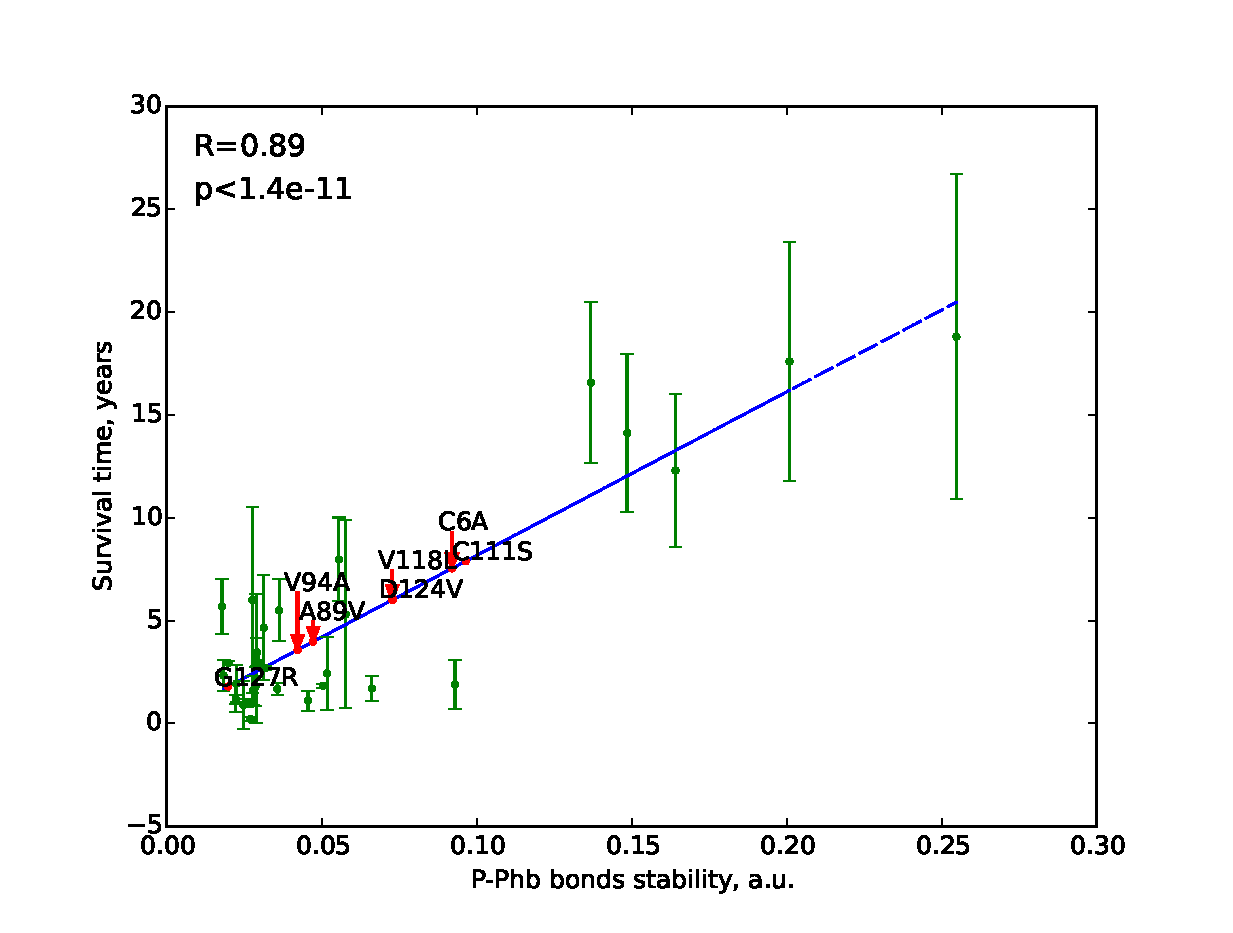
\includegraphics [width=0.75\linewidth] {md_ST_a}
  \caption{Зависимость между продолжительностью жизни пациентов и стабильностью связей в модели \modelpphb{}.}
  \label{img:md_ST_a}
\end{figure}

\begin{figure}[ht]
  \center
  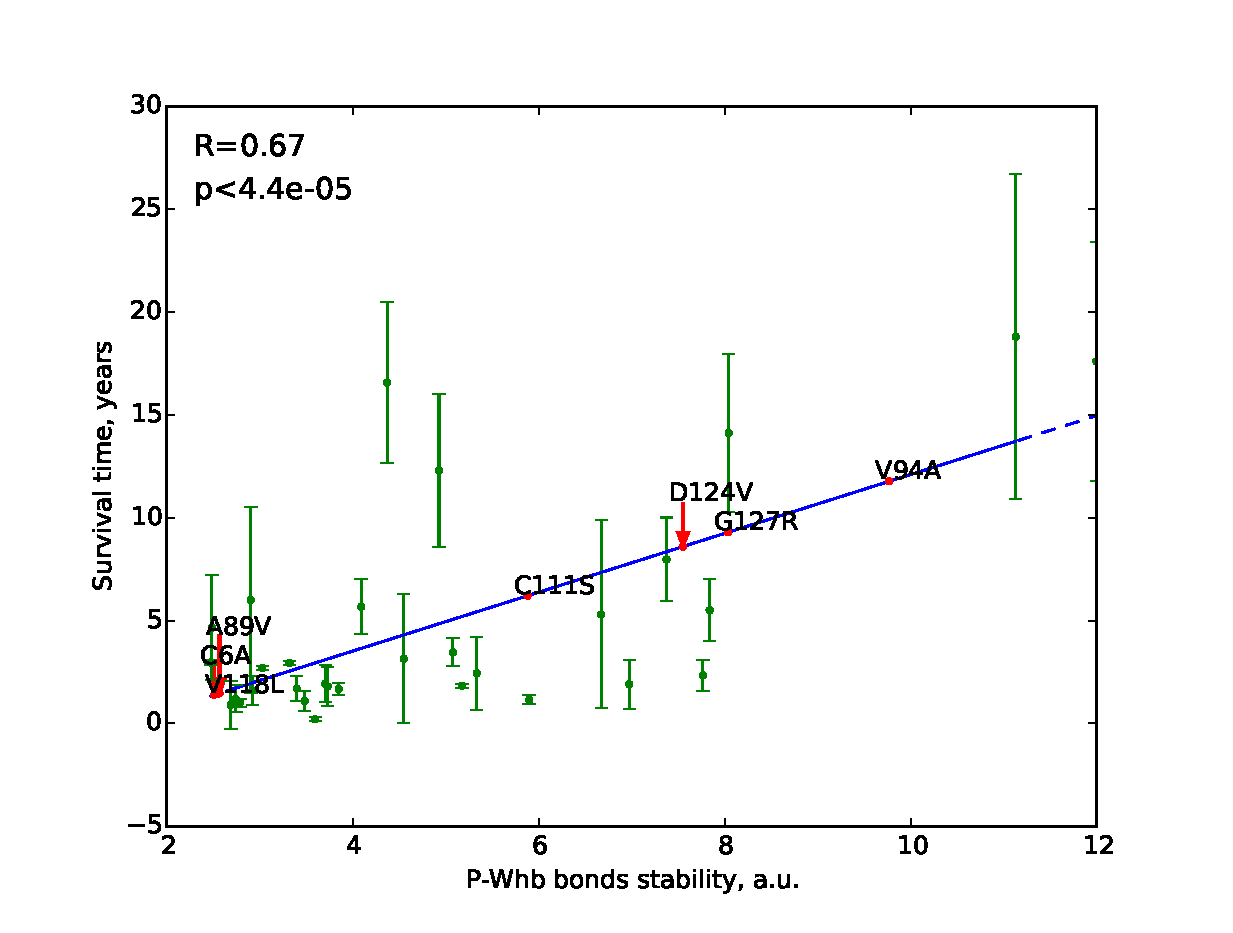
\includegraphics [width=0.75\linewidth] {md_ST_b}
  \caption{Зависимость между продолжительностью жизни пациентов и стабильностью связей в модели \modelpwhb{}.}
  \label{img:md_ST_b}
\end{figure}

\begin{figure}[ht]
  \center
  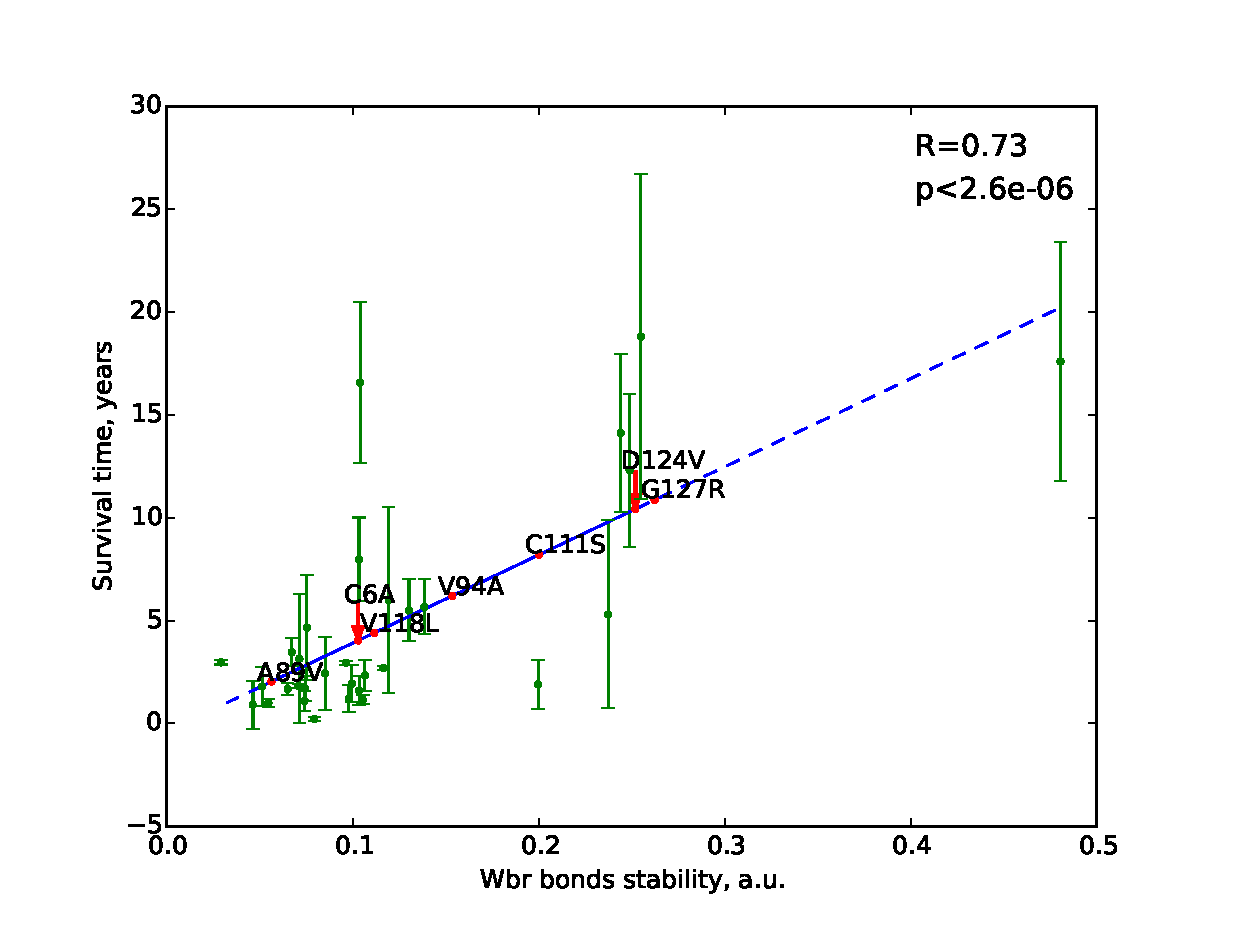
\includegraphics [width=0.75\linewidth] {md_ST_c}
  \caption{Зависимость между продолжительностью жизни пациентов и стабильностью связей в модели \modelwbr{}.}
  \label{img:md_ST_c}
\end{figure}

Графики зависимости для каждой индивидуальной модели \modelpphb{}, \modelpwhb{} и \modelwbr{} между продолжительностью жизни пациентов и стабильностью связей  показаны на Рис. \ref{img:md_ST_a}, \ref{img:md_ST_b}, \ref{img:md_ST_c}. Оказалось, что наилучшей моделью из трёх является модель  \modelpphb{} ($R=0.89$, $p<10^{-10}$). Уравнение регрессии имело вид: $\widehat{ST}^m = 79.53*O_{m, K}^{\text{\modelpphb{}}}+0.22$. Оставшиеся две модели расположились друг относительно друга по коэффициенту корреляции в следующем порядке:  \modelwbr{} ($R=0.73$, $p<0.00001$) и \modelpwhb{} ($R=0.67$, $p<0.0001$). 

Дополнительно были построены две комбинированные модели с использованием линейной множественной регрессии (далее--\modelCLS{}) и метода Random forest \cite{Breiman2001} (далее--\modelCRF{}), учитывающие стабильность одновременно трёх типов связей (водородных связей между атомами белка, атомами белка и атомами молекул воды и водных мостиков). Метод Random forest был применён потому, что он учитывает сложные независимые взаимные связи между используемыми предикторами \cite{Karatayev2015}. Ещё одной причиной стала неявная перекрёстная проверка, реализующаяся данным методом.

\begin{figure}[ht]
  \center
  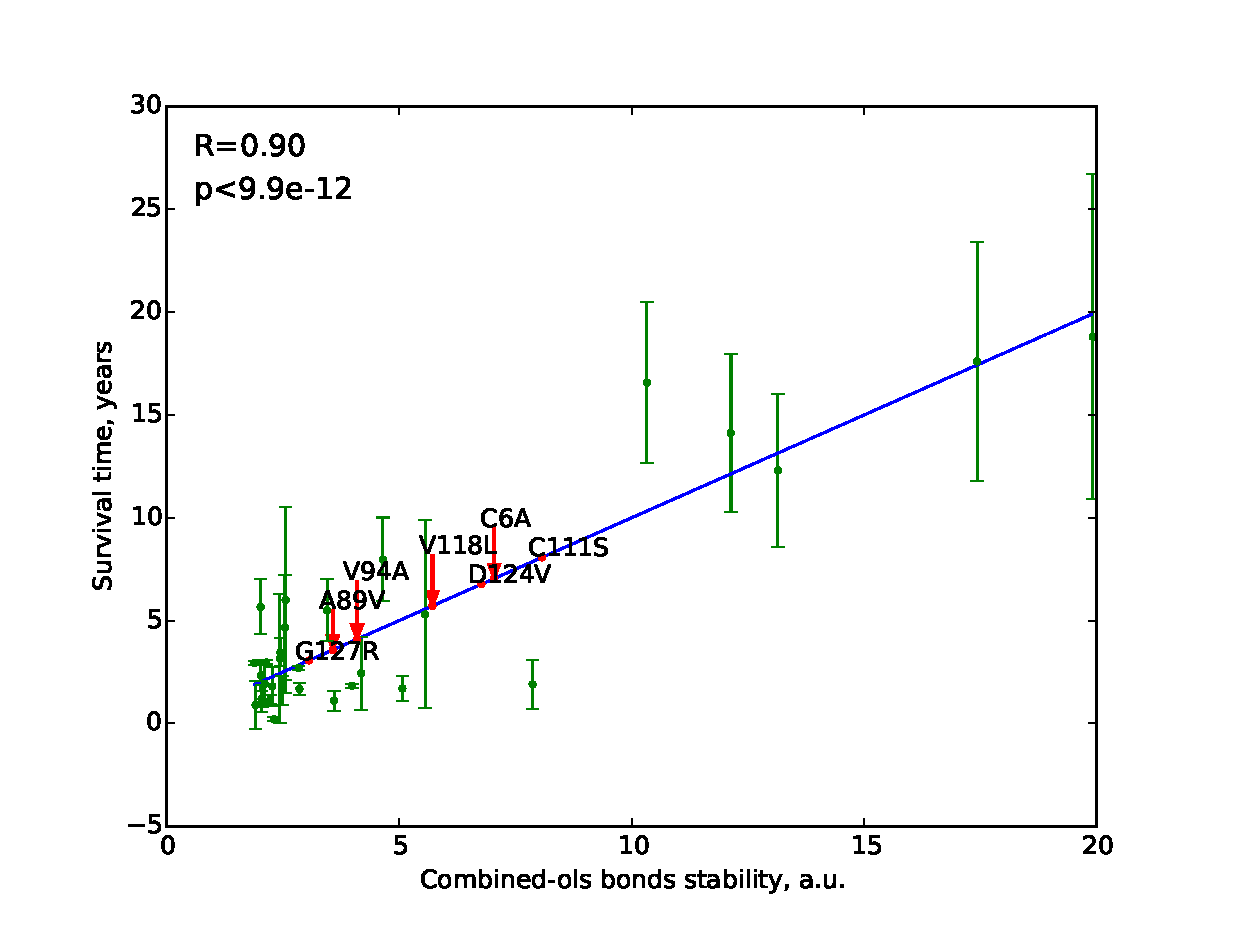
\includegraphics [width=0.75\linewidth] {md_STc_a}
  \caption{Зависимость между продолжительностью жизни пациентов и стабильностью связей в модели \modelCLS{}.}
  \label{img:md_STc_a}
\end{figure}

\begin{figure}[ht]
  \center
  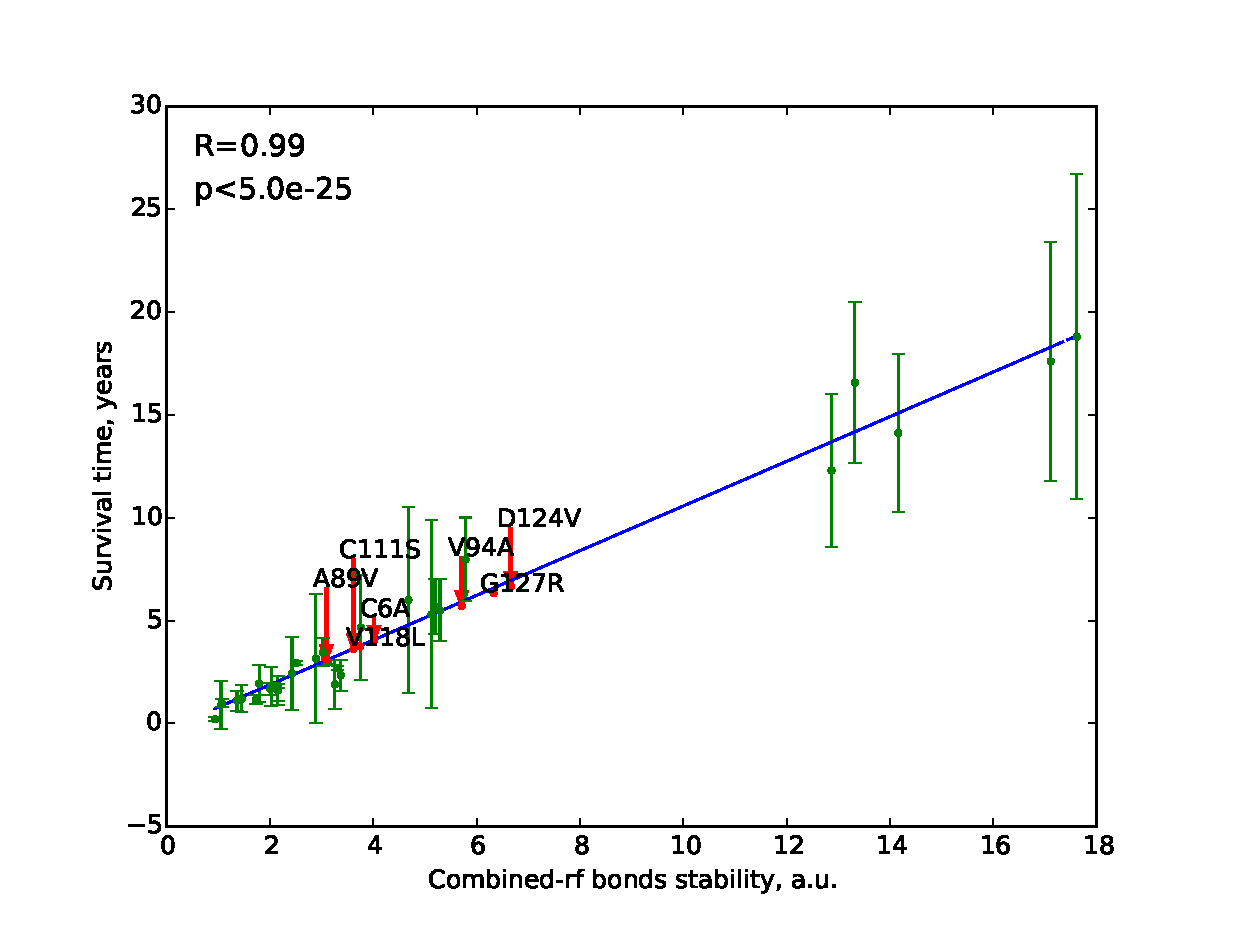
\includegraphics [width=0.75\linewidth] {md_STc_b}
  \caption{Зависимость между продолжительностью жизни пациентов и стабильностью связей в модели \modelCRF{}.}
  \label{img:md_STc_b}
\end{figure}

Коэффициенты множественной корреляции для \modelCLS{} и \modelCRF{} составили 0.90 ($p < 10^{-11}$) и 0.99 ($p < 10^{-24}$), соответственно (см. Рис. \ref{img:md_STc_a}, \ref{img:md_STc_b}). Модель \modelCLS{} описывалась следующим уравнением:  $\widehat{ST}^m = 71.38*O_{m, K}^{\text{\modelpphb{}}}+0.04*O_{m, K}^{\text{\modelpwhb{}}}+5.85*O_{m, K}^{\text{\modelwbr{}}}-0.24$. Модель \modelCRF{}, как оказалось, имеет более высокий множественный коэффициент корреляции. Факторы, исследованные при построении данной модели имели следующие характеристики важности: 0.75 (\modelpphb{}), 0.09 (\modelpwhb{}) и 0.16 (\modelwbr{}), что согласуется со множителями в уравнении модели \modelCLS{}.

Из коэффициентов множественной корреляции видно, что добавление факторов \modelpwhb{} и \modelwbr{} к \modelpphb{} лишь незначительно улучшает множественную корреляцию. Это происходит, по-видимому, из-за того, что между всеми тремя факторами есть зависимость. Для того, чтобы проверить, есть ли согласие между номерами аминокислотных остатков, формирующих значимые связи, на которые, в свою очередь, опираются предсказания каждой из моделей \modelpphb{}, \modelpwhb{} и \modelwbr{}, были построены, соответственно, три таблицы сопряжённости. Согласие между номерами таких остатков в моделях \modelpphb{} и \modelpwhb{} было значимо на уровне $p < 0.0026$ по точному тесту Фишера. Между \modelpwhb{} и \modelwbr{} такая значимость была $p < 0.0032$, а между \modelpphb{} и \modelwbr{}--$p < 0.006$. Из этого был сделан вывод о том, что, действительно, факторы \modelpphb{}, \modelpwhb{} и \modelwbr{} во множественных регрессионных моделях \modelCLS{} и \modelCRF{} зависимы между собой. Однако анализ межмолекулярных взаимодействий белка с водой, проведённый при построении моделей \modelpwhb{} и \modelwbr{} позволил лучше понять молекулярные механизмы нарушений в структуре мутантных форм SOD1, приводящих к развитию заболевания.

\begin{figure}[ht]
  \center
  \includegraphics [width=0.75\linewidth] {SOD1_hb13}
  \caption{Пространственное расположение первых 13 водородных связей, образованных между аминокислотными остатками белка SOD1 (PDBID: 2V0A).}
  \label{img:SOD1_hb13}
\end{figure}

В ходе анализа была получена детальная информация о различных типах связей, образующихся в белке SOD1, использованных для предсказания продолжительности жизни пациентов. Были проанализированы как связи, сформированные между аминокислотными остатками, удалёнными друг от друга в первичной структуре белка, так и между сближенными (например, водородная связь между остатком 77 и 102, а также водородная связь между 135 и 138). Расположение части из этих связей в пространственной структуре белка показано на Рис. \ref{img:SOD1_hb13}.

\begin{figure}[ht]
  \center
  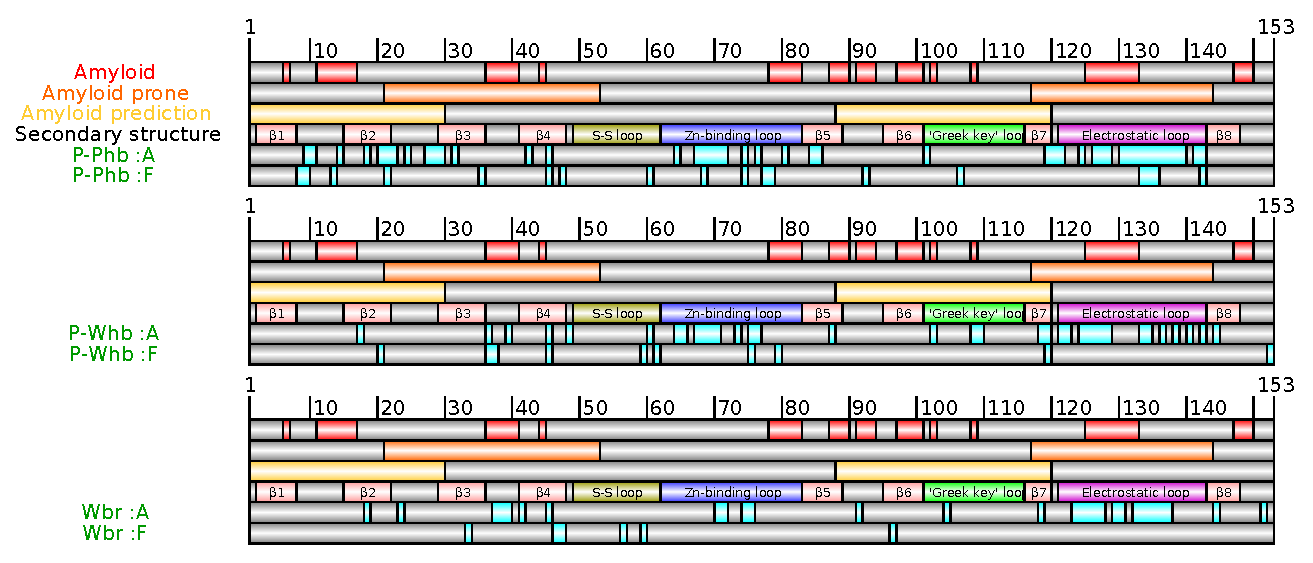
\includegraphics [width=0.75\linewidth] {SOD1_seq_anno}
  \caption{Аннотация первичной структуры SOD1. Каждая из трёх диаграмм состоит из шести строк, отражающих: (1) области, известные как агрегирующие; (2) области, подверженные агрегации; (3) области, предсказанные как агрегирующие; (4) вторичная структура SOD1; (5) области субъединицы A, в которых обнаружены важные межатомные связи; (6) аналогичные области субъединицы F. Подписью <<Amyloid>> красного цвета выделены остатки, которые, как известно из литературных данных \cite{Elam2003,Wright2013,Banci2009,Antonyuk2005}, содержатся в интерфейсе при связывании амилоидов SOD1. Подписи <<Amyloid prone>> оранжевого цвета выделяет те области белка, которые подвержены агрегации \cite{Durazo2009}, а <<Amyloid prediction>> жёлтого цвета--для которых сделано подобное предсказание \cite{Wright2013}. Подпись <<Secondary structure>> выделяет группу аминокислотных остатков, характеризующих функциональные области белка и элементы его вторичной структуры. Вторичная структура (строка 4) закодирована цветами: розовый--$\beta$-листы, жёлтый--дисульфидная петля, синий--Zn-связывающая петля, зелёный--петля типа <<Greek key>>, фиолетовый--электростатическая петля.}
  \label{img:SOD1_seq_anno}
\end{figure}

На Рис. \ref{img:SOD1_seq_anno} показаны аминокислотные остатки, участвующие в формировании связей, использованных для построения регрессионных моделей \modelpphb{}, \modelpwhb{}, и \modelwbr{}. Только те остатки, в которых время существования межатомных связей (водородные связи между атомами самого белка, между атомами белка и атомами молекул воды, а также водные мостики) в траектории МД с наибольшим коэффициентом коррелировало с продолжительностью жизни пациентов ($|R_k| > |R_{th}|$), учитывались при построении каждой из трёх диаграм. Было показано, что данные $K$ важных для регрессионных моделей связей стабилизированы или дестабилизированы в мутантах по сравнению с SOD1 дикого типа. Всего найдено 69, 81 и 19 связей каждого типа из \modelpphb{}, \modelpwhb{}, и \modelwbr{}, соответственно.
Для проверки согласия между важными областями в структуре белка SOD1, определёнными в процессе построения регрессионных моделей, и известными из литературы областями, участвующими в агрегации (см. Рис. \ref{img:SOD1_seq_anno}), был применён точный тест Фишера. Были построены таблицы сопряжённости, по которым вычислялась значимость взаимосвязи между номерами важных аминокислотных остатков для каждой из трёх моделей (\modelpphb{}, \modelpwhb{} и \modelwbr{}) и номерами остатков в каждом из литературных свидетельств о связи белка с агрегацией (<<Amyloid>>, <<Amyloid prone>> и <<Amyloid prediction>>). Значение p ниже, чем 0.05 считалось значимым для указанной взаимосвязи, а соответствующее предсказание--согласующимся с литературными данными. 

В результате проверки обнаружено, что остатки субъединицы A белка SOD1, предсказанные как важные для модели \modelpphb{}, по точному тесту Фишера значимо ($p < 0.001$) взаимосвязаны с аминокислотными остатками, подверженными агрегации (<<Amyloid prone>>), как указано в \cite{Durazo2009}. Со значимостью $p < 0.05$ остатки субъединицы A для модели \modelpwhb{} лежат в областях SOD1, подверженных агрегации (<<Amyloid prone>>, в \cite{Durazo2009}) и предсказанных ранее (<<Amyloid prediction>>), как указано в \cite{Wright2013}. Кроме того, со значимостью $p < 0.05$ важные остатки субъединицы A для \modelpwhb{} содержатся в упорядоченных элементах вторичной структуры белка SOD1 (<<Secondary structure>>). Наконец, остатки субъединицы A, важные для модели \modelwbr{}, как оказалось, лежат в областях SOD1, подверженных агрегации (<<Amyloid prone>>, в \cite{Durazo2009} и предсказанных ранее (<<Amyloid prediction>>, в \cite{Wright2013}).

\section{Исследование моделей \modelpphb{}, \modelpwhb{} и \modelwbr{}} \label{sect_MD_analysis}

Для статистической проверки точности моделей \modelpphb{}, \modelpwhb{} и \modelwbr{} по предсказанию времени жизни пациентов был применён метод bootstrap. Для этого данные по продолжительности жизни пациентов, включающие в себя информацию об $M$ мутантах (множество $\mathfrak{M}$) были разбиты на обучающую ($\frac{2}{3}$ элементов $\mathfrak{M}$) и тестовую выборку ($\frac{1}{3}$ элементов $\mathfrak{M}$). Было проведено $10^5$ шагов bootstrap, на каждом из которых оценивалась величина стандартной ошибки $S$, как средний квадрат разности между полученными с помощью модели предсказаниями и опубликованными в литературе временами жизни пациентов, носителей соответствующих мутаций.
Для дополнительной верификации описанных выше исходных моделей, было проведено их сравнение со случайными моделями, построенными на основе случайного выбора $K$ важных связей. Для случайных моделей рассчитывалась та же мера $S$.

Полученные распределения величины $S$ для исходных моделей сравнивались с распределением $S$, рассчитанным для случайных моделей, с применением непараметрических критериев $\chi^2$, Краскела-Уоллиса \cite{Kruskal1952}, Колмогорова-Смирнова \cite{Kolmogorov1933,Smirnov1948} и Манна-Уитни-Вилкоксона \cite{Mann1947,Wilcoxon1945}. Для иллюстрации отличия исходных моделей от случайных методом BCa (bias-corrected and accelerated bootstrap) \cite{efron_better_1987} рассчитывался 95\% доверительный интервал для среднего значения величины $S$.

\begin{figure}[ht]
  \center
  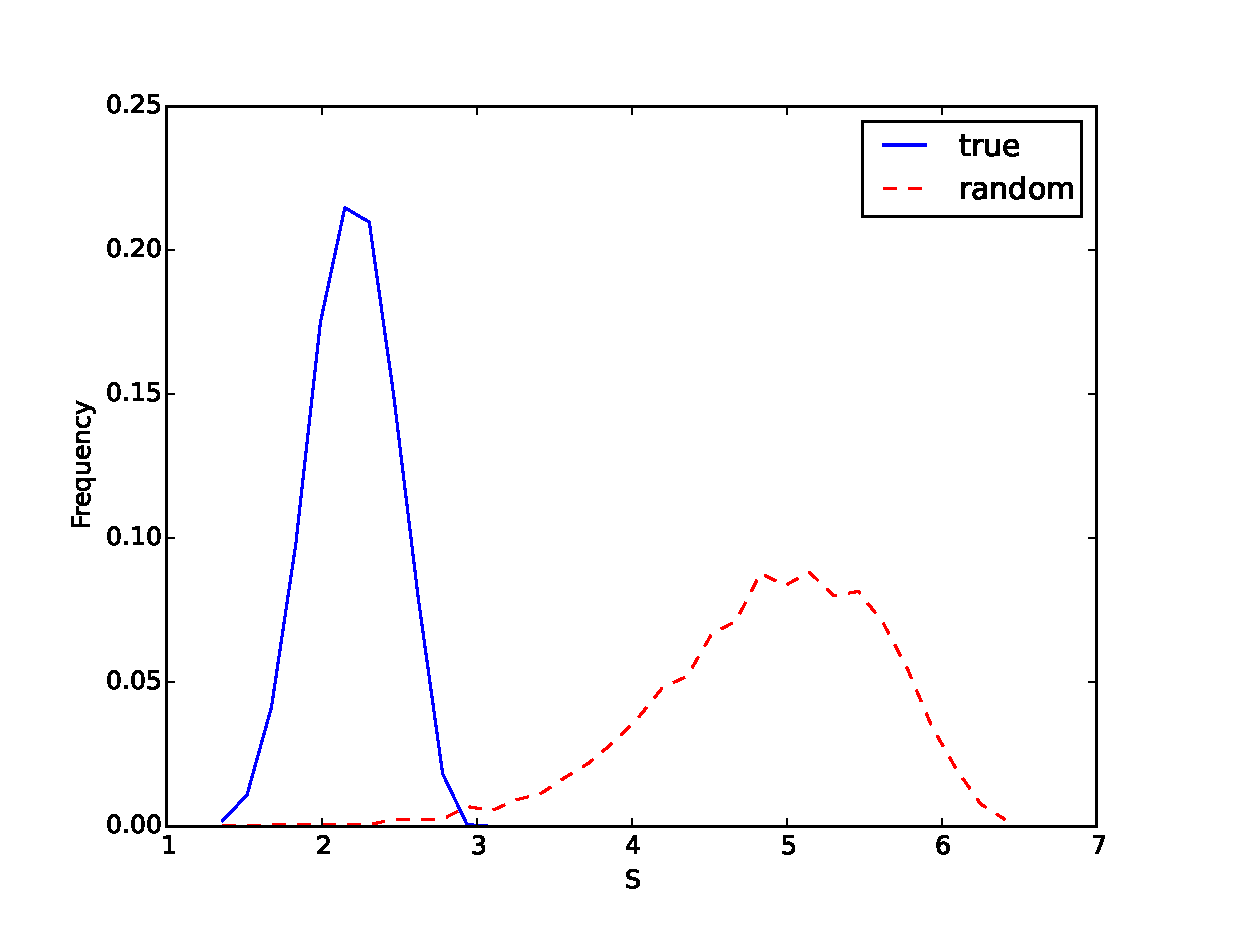
\includegraphics [width=0.75\linewidth] {md_distr_a}
  \caption{Распределения величины $S$, ожидаемые по случайным причинам и наблюдаемые в исходной модели \modelpphb{}.}
  \label{img:md_distr_a}
\end{figure}

\begin{figure}[ht]
  \center
  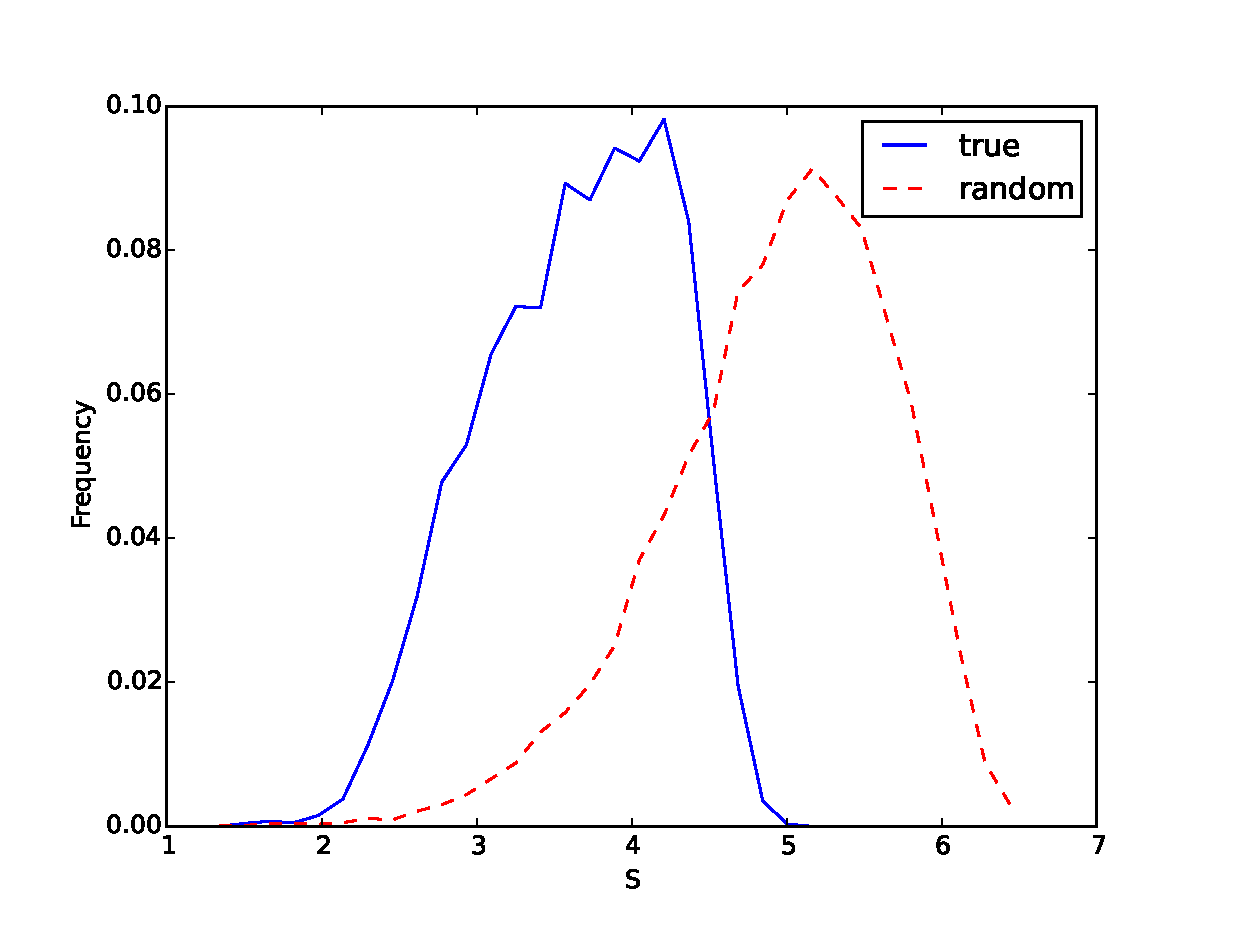
\includegraphics [width=0.75\linewidth] {md_distr_b}
  \caption{Распределения величины $S$, ожидаемые по случайным причинам и наблюдаемые в исходной модели \modelpwhb{}.}
  \label{img:md_distr_b}
\end{figure}

\begin{figure}[ht]
  \center
  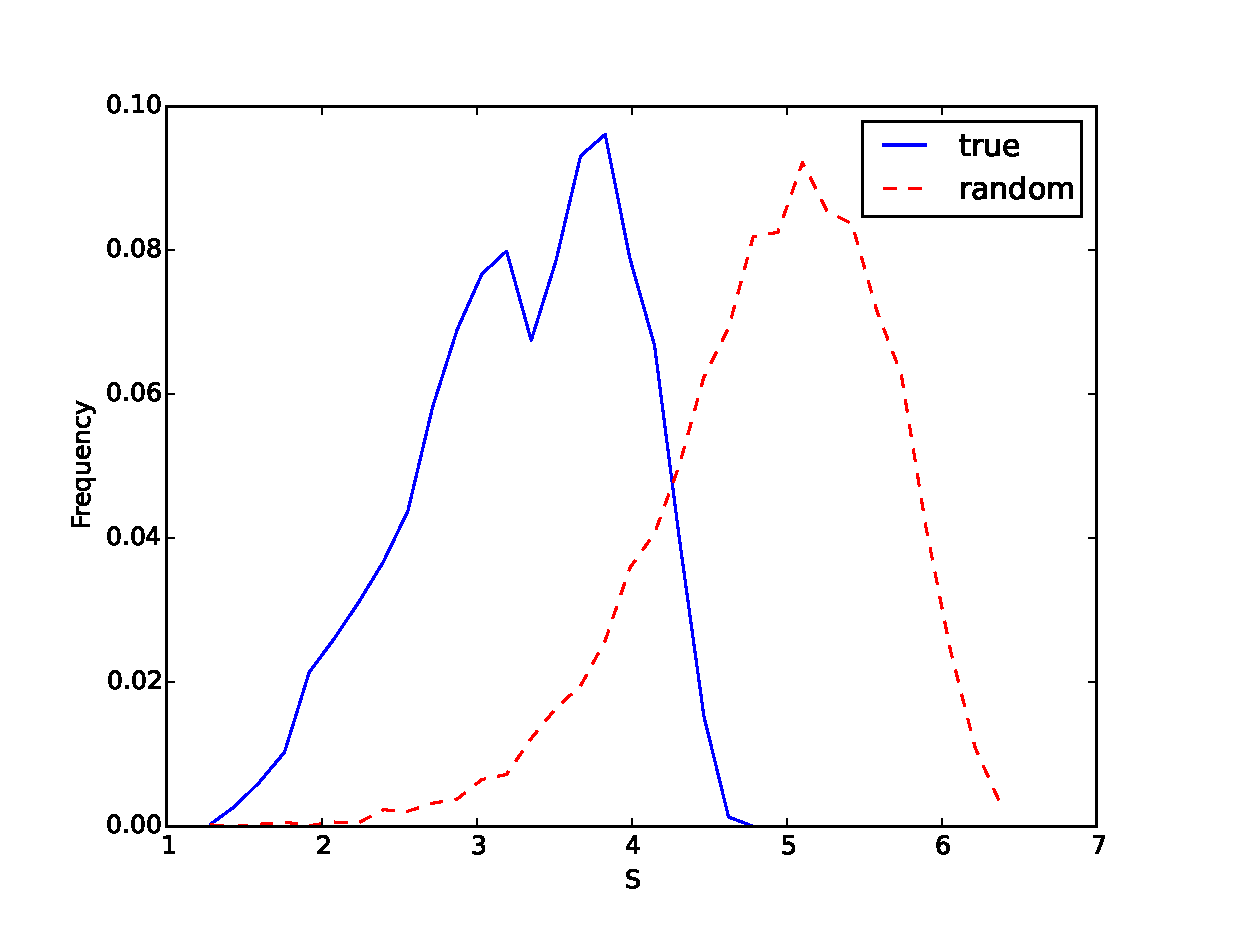
\includegraphics [width=0.75\linewidth] {md_distr_c}
  \caption{Распределения величины $S$, ожидаемые по случайным причинам и наблюдаемые в исходной модели \modelwbr{}.}
  \label{img:md_distr_c}
\end{figure}

\begin{table} [htbp]%
    \centering
	\caption{Отличие между распределением величины, ожидаемым по случайным причинам и наблюдаемым в исходных моделях.}\label{tbl:models_distr}% label всегда желательно идти после caption
%    \renewcommand{\arraystretch}{1.5}%% Увеличение расстояния между рядами, для улучшения восприятия.
    \begin{SingleSpace}
	\begin{tabular}{@{}@{\extracolsep{20pt}}lll@{}} %Вертикальные полосы не используются принципиально, как и лишние горизонтальные (допускается по ГОСТ 2.105 пункт 4.4.5) % @{} позволяет прижиматься к краям
        \toprule     %%% верхняя линейка
	Модель & $S$ для исходных моделей & $S$ для случайных моделей \\
        \midrule %%% тонкий разделитель. Отделяет названия столбцов. Обязателен по ГОСТ 2.105 пункт 4.4.5 
	\modelpphb{}	&	$2.3\pm0.005$	&	$5.0\pm0.014$ \\
	\modelpwhb{}	&	$3.7\pm0.012$	&	$5.0\pm0.015$ \\
	\modelwbr{}	&	$3.4\pm0.013$	&	$5.0\pm0.015$ \\
        \bottomrule %%% нижняя линейка
	\end{tabular}%
   	\end{SingleSpace}
\end{table}

Результаты сравнения индивидуальных моделей со случайными моделями (см. раздел \ref{chapt2}) приведены в Таблице \ref{tbl:models_distr} и на Рис. \ref{img:md_distr_a}, \ref{img:md_distr_b}, \ref{img:md_distr_c}.  Как видно из таблицы и рисунка, средние значения величины $S$ для каждой из моделей статистически значимо отличаются от ожидаемых по случайным причинам. Кроме того, согласно непараметрическим критериям ($\chi^2$, Краскела-Уоллиса, Колмогорова-Смирнова и Манна-Уитни-Вилкоксона), распределения величины $S$ исходных моделей также значимо отличались ($p < 0.001$) от случайных моделей. Сравнение показало, что найденные $K$ связей позволяют основанным на их параметрах регрессионным моделям быть существенно отличными от случайных моделей.

\section{Предсказание продолжительности жизни пациентов с мутациями в SOD1, для которых сведения в литературе неполны} \label{sect_MD_prediction}

\begin{table} [htbp]%
    \centering
	\caption{Предсказания моделей  \modelpphb{}, \modelpwhb{}, \modelwbr{}, \modelCLS{}, \modelCRF{} для мутаций с неполной информацией о продолжительности жизни пациентов--их носителей, выраженные в годах.}\label{tbl:models_pred}% label всегда желательно идти после caption
%    \renewcommand{\arraystretch}{1.5}%% Увеличение расстояния между рядами, для улучшения восприятия.
    \begin{SingleSpace}
	\begin{tabular}{@{}@{\extracolsep{20pt}}llllll@{}} %Вертикальные полосы не используются принципиально, как и лишние горизонтальные (допускается по ГОСТ 2.105 пункт 4.4.5) % @{} позволяет прижиматься к краям
        \toprule     %%% верхняя линейка
	Мутация & \modelpphb{} & \modelpwhb{} & \modelwbr{} & \modelCLS{} & \modelCRF{} \\
        \midrule %%% тонкий разделитель. Отделяет названия столбцов. Обязателен по ГОСТ 2.105 пункт 4.4.5 
	Цис6Ала	& 7.53 & 1.39 & 4.03 & 7.04 & 4.01 \\
	Ала89Вал	& 3.98 & 1.47 & 2.03 & 3.57 & 3.09 \\
	Вал94Ала	& 3.57 & 11.77 & 6.2 & 4.09 & 5.71 \\
	Цис111Сер	& 7.89 & 6.21 & 8.2 & 8.07 & 3.62 \\
	Вал118Лей	& 6.0 & 1.46 & 4.4 & 5.71 & 3.57 \\
	Асп124Вал	& 6.02 & 8.6 & 10.42 & 6.77 & 6.66 \\
	Гли127Арг	& 1.8 & 9.29 & 10.86 & 3.06 & 6.33 \\
        \bottomrule %%% нижняя линейка
	\end{tabular}%
   	\end{SingleSpace}
\end{table}

Построенные модели были применены для предсказания времён жизни пациентов с четырьмя точечными мутациями (Ала89Вал, Вал118Лей, Асп124Вал и Гли127Арг (Рис.  \ref{md_ST_a}, \ref{md_ST_b}, \ref{md_ST_c} и \ref{md_STc_a}, \ref{md_STc_b})), данные о которых в литературе неполны. Для двоих из этих пациентов (с мутациями Ала89Вал и Асп124Вал) точных сведений о продолжительности жизни не было известно. О пациенте с мутацией Асп124Вал известно, что он жил более 2 лет \cite{Wang2008}. Заболевание у другого пациета с мутацией Ала89Вал длилось около 6 лет \cite{Sato2005}. На момент публикации этих авторов пациент предположительно был ещё жив. Кроме того, в работе \cite{Wang2008} приведены сведения о том, что пациенты с Ала89Вал имеют продолжительность жизни в среднем более 3.8 лет. Также было известно, что один пациент--носитель мутации Вал118Лей жил около 8 лет \cite{Shimizu2000}. Для мутации Гли127Арг в работе \cite{Holmoy2010} были приведены сведения об одном пациенте, продолжительность жизни которого составила 7 месяцев. Данные мутации не вносились в обучающую выборку. Как видно из Таблицы \ref{tbl:models_pred}, предсказания имели хорошее согласие с имеющейся о данных мутациях информацией о продолжительности жизни пациентов.

Предсказания также были сделаны ещё для двух мутаций (Цис6Ала, Цис111Сер), для которых нет литературных данных о времени жизни пациентов \cite{Lepock1990}.
Дополнительно была промоделирована мутация Вал94Ала. В результате моделирования оказалось, что остаток Вал94 образует водородные связи с остатками Асп90 и Лей38, замены в которых, как известно, приводят к БАС.

Оказалось, что все эти мутации распределились от 1.3 до 11.8 лет на шкале времени жизни пациентов.

\section{Оценка точности предсказаний продолжительности жизни на основе моделирование выборки пациентов} \label{sect_MD_crossvalidation}

Для построения регрессионных моделей была использована изначально ограниченная информация о продолжительности жизни пациентов. Это было вызвано тем, что в использованных источниках данных содержались сведения только о средней продолжительности жизни группы пациентов с определённой мутацией, стандартное отклонение этой величины от среднего и число пациентов в группе \cite{Wang2008}. В таком случае предсказания моделей, построенных на основе среднего значения, также будут иметь характер средних значений. Другими словами, если, например, модель \modelpphb{} предсказывает для пациента с мутацией Гли127Арг продолжительность жизни 1.8 года, это означает, что, в среднем, такие пациенты после наступления болезни будут жить указанное время. При этом остаётся неизвестной нижняя и верхняя граница предсказанного значения.

Для преодоления данного недостатка при построении регрессионных моделей использовался подход моделирования генеральной совокупности. В рамках этого подхода для каждой мутации случайным образом строилась обучающая выборка продолжительностей жизни с учётом информации о среднем значении, стандартном отклонении и количестве пациентов. Предполагалось нормальное распределение случайной величины, так как в источниках данных сведений о распределении не было указано. 

\begin{table} [htbp]%
    \centering
	\caption{Предсказания моделей  \modelpphb{}, \modelpwhb{}, \modelwbr{}, \modelCLS{}, \modelCRF{} с учётом дисперсии в данных обучающей выборки, выраженные в годах.}\label{tbl:models_pred_disp}% label всегда желательно идти после caption
%    \renewcommand{\arraystretch}{1.5}%% Увеличение расстояния между рядами, для улучшения восприятия.
    \begin{SingleSpace}
	\begin{tabular}{@{}@{\extracolsep{20pt}}llllll@{}} %Вертикальные полосы не используются принципиально, как и лишние горизонтальные (допускается по ГОСТ 2.105 пункт 4.4.5) % @{} позволяет прижиматься к краям
        \toprule     %%% верхняя линейка
	Мутация & \modelpphb{} & \modelpwhb{} & \modelwbr{} & \modelCLS{} & \modelCRF{} \\
        \midrule %%% тонкий разделитель. Отделяет названия столбцов. Обязателен по ГОСТ 2.105 пункт 4.4.5 
	Цис6Ала & $7.5\pm1.1$ & $1.0\pm0.6$ & $4.2\pm0.3$ & $6.4\pm1.2$ & $3.9\pm1.3$ \\ 
	Ала89Вал & $3.8\pm0.3$ & $1.1\pm0.6$ & $2.3\pm0.5$ & $3.3\pm0.8$ & $2.9\pm1.1$ \\
	Вал94Ала & $3.4\pm0.3$ & $12.1\pm1.9$ & $6.3\pm0.7$ & $4.7\pm1.3$ & $7.4\pm1.1$ \\
	Цис111Сер & $7.9\pm1.2$ & $6.2\pm0.6$ & $8.2\pm1.1$ & $7.9\pm1.1$ & $2.6\pm2.5$ \\
	Вал118Лей & $5.9\pm0.7$ & $1.1\pm0.6$ & $4.6\pm0.4$ & $5.3\pm0.7$ & $4.1\pm1.3$ \\
	Асп124Вал & $5.9\pm0.7$ & $8.7\pm1.2$ & $10.3\pm1.6$ & $6.9\pm1.7$ & $6.0\pm5.5$ \\
	Гли127Арг & $1.6\pm0.5$ & $9.5\pm1.3$ & $10.7\pm1.7$ & $3.8\pm2.8$ & $6.4\pm4.7$ \\
        \bottomrule %%% нижняя линейка
	\end{tabular}%
   	\end{SingleSpace}
\end{table}

С использованием построенных обучающих выборок продолжительностей жизни пациентов с соответствующими мутациями были исследованы предсказания исходных регрессионных моделей \modelpphb{}, \modelpwhb{}, \modelwbr{}, \modelCLS{} и \modelCRF{}. Для каждой модели было рассчитано среднее значение предсказанной продолжительности жизни пациента с определённой мутацией и стандартное отклонение этого значения от среднего (см. Таблицу \ref{tbl:models_pred_disp}). В качестве тестовой выборки выступал список мутаций, для которых в литературе нет данных о продолжительности жизни пациентов. Предсказания получались применением соответствующих регрессионных уравнений к обучающей выборке. Всего было сформировано 10000 обучающих выборок.

\section{Выводы} \label{sect_MD_implications}

Было сделано предположение, что, метастабильные конформационные состояния белков, при которых они подвержены агрегации, определяются как стабилизацией, так и дестабилизацией структуры белка в результате мутаций. В настоящей работе показано, что в локальной дестабилизации белка участвуют чаще те аминокислотные остатки, которые находятся в той или иной функциональной области белка. Выявлена важная роль водородных связей и водных мостиков в увеличении вероятности локальной дестабилизации его структуры. 

Были построены регрессионные модели, связывающие конформационные свойства мутантов SOD1, носители которых проявляют признаки БАС со временем жизни таких пациентов. Показано, что время жизни пациентов с момента диагностики признаков заболевания хорошо коррелирует с конформационными особенностями мутантных белков SOD1 этих пациентов. Коэффициет корреляции продолжительности жизни со временем существования внутримолекулярных водородных связей составил 0.89 ($p<10^{-10}$). Со временем существования водородных связей между белком и окружающими его молекулами воды--0.73 ($p<0.00001$). Со временем существования водных мостиков--0.67 ($p<0.0001$). Коэффициент множественной корреляции, построенной на основе всех трёх факторов оказался равен 0.9 ($p<10{-11}$). Показано, что в локальной дестабилизации белка SOD1 чаще всего участвуют аминокислотные остатки, расположенные в его функциональных областях. Была выявлена важная роль водородных связей и водных мостиков в увеличении вероятности локальной дестабилизации белковой структуры. С помощью построенных моделей предсказано, что мутация Вал94Ала может вызывать БАС. Предсказана продолжительность жизни пациентов с этой мутацией, если они будут обнаружены: от 3.57 до 11.77 лет. Мутация Вал94Ала может использоваться для генотипирования пациентов с БАС.

\todo{Построенные регрессионные модели позволили обнаружить существенные для предсказания продолжительности жизни участки в структуре белка SOD1, мутации в которых изменяют время существования водородных связей и водных мостиков. Данный подход позволяет найти корреляцию между микроскопическими свойствами белков (количество водородных связей внутри белка, водородных связей остатков белка с молекулами воды и водных мостиков, время их существования и т. д.) и макроскопическими свойствами (термостабильность, константа ассоциации с лигандами и т.д.). Сделано предположение о том, что окружающие SOD1 молекулы воды в большой степени влияют на динамику водородных связей внутри белка и могут выступать в качестве важного фактора в развитии БАС.}
